\documentclass[tikz,border=4pt]{standalone}
\usepackage{tikz}
\usetikzlibrary{positioning,calc,arrows.meta}
\usepackage{amsmath}

\begin{document}
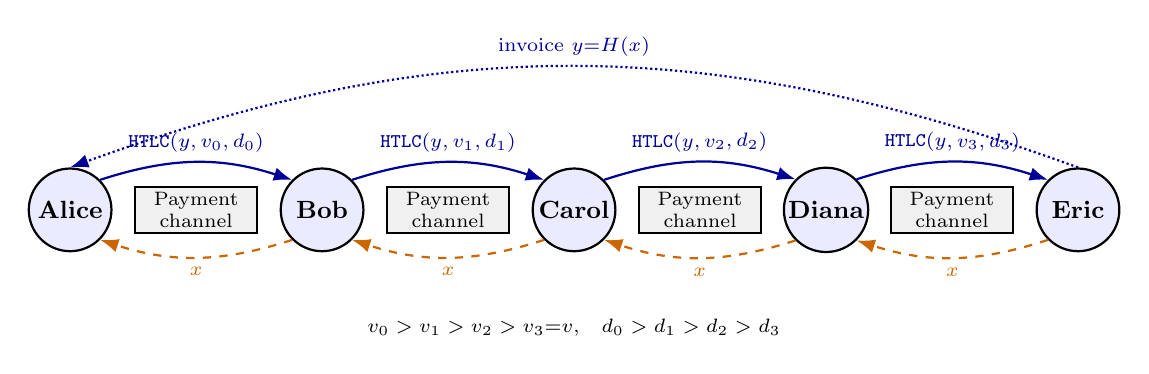
\begin{tikzpicture}[
  x=1cm, y=1cm,
  party/.style={circle, draw, thick, fill=blue!8,
                minimum size=1.05cm, font=\small\bfseries, inner sep=1pt},
  ch/.style={draw, thick, fill=gray!12, minimum height=0.38cm, minimum width=1.55cm,
             font=\scriptsize, align=center, inner sep=2pt},
  arrL/.style={-{Latex}, thick, blue!60!black},
  arrR/.style={-{Latex}, thick, orange!80!black, dashed},
  lab/.style={font=\scriptsize}
]

\node[party] (A) at (0,0)    {Alice};
\node[party] (B) at (3.2,0)  {Bob};
\node[party] (C) at (6.4,0)  {Carol};
\node[party] (D) at (9.6,0)  {Diana};
\node[party] (E) at (12.8,0) {Eric};

\node[ch] at ($(A)!0.5!(B)$) {Payment\\channel};
\node[ch] at ($(B)!0.5!(C)$) {Payment\\channel};
\node[ch] at ($(C)!0.5!(D)$) {Payment\\channel};
\node[ch] at ($(D)!0.5!(E)$) {Payment\\channel};

% Lock (HTLC) above
\draw[arrL] (A.north east) to[bend left=18] node[lab, above, sloped] {\texttt{HTLC}$(y,v_0,d_0)$} (B.north west);
\draw[arrL] (B.north east) to[bend left=18] node[lab, above, sloped] {\texttt{HTLC}$(y,v_1,d_1)$} (C.north west);
\draw[arrL] (C.north east) to[bend left=18] node[lab, above, sloped] {\texttt{HTLC}$(y,v_2,d_2)$} (D.north west);
\draw[arrL] (D.north east) to[bend left=18] node[lab, above, sloped] {\texttt{HTLC}$(y,v_3,d_3)$} (E.north west);

% Release (preimage) below
\draw[arrR] (E.south west) to[bend left=18] node[lab, below, sloped] {$x$} (D.south east);
\draw[arrR] (D.south west) to[bend left=18] node[lab, below, sloped] {$x$} (C.south east);
\draw[arrR] (C.south west) to[bend left=18] node[lab, below, sloped] {$x$} (B.south east);
\draw[arrR] (B.south west) to[bend left=18] node[lab, below, sloped] {$x$} (A.south east);

% Invoice hint
\draw[arrL, densely dotted] (E.north) to[bend right=20]
  node[lab, above, pos=0.5] {invoice $y{=}H(x)$} (A.north);

\node[lab] at ($(A)!0.5!(E) + (0,-1.5)$) {$v_0>v_1>v_2>v_3{=}v$,\quad $d_0>d_1>d_2>d_3$};

\end{tikzpicture}
\end{document}
